\documentclass[11pt,a4paper,oneside]{article}

\usepackage{euler,amsthm,amsmath,amsfonts,graphicx,epigraph,indentfirst,enumerate,comment,listings,fontspec,color,subcaption,listings}
\usepackage{xeCJK}
\usepackage{hw}
\usepackage{pythonhighlight}

\renewcommand{\hwtitle} {CS217 Homework 1}	
\renewcommand{\hwauthor}{Akina}
\renewcommand{\hwdate}{\today}

\begin{document}
\title{\hwtitle}
\author{\hwauthor}
\date{\hwdate}
\maketitle

\section*{Bit Complexity of Euclid's Algorithm}
We have proved that Euclid's algorithm for computing $\gcd(a,b)$ makes at most
$O(\log a)$ iterations. What is the overall running time? Each iteration computes
$u \mod v$ for some integers. This can be done by integer division. What is its running time?
There are very sophisticated algorithms, but python probably does not come with them. 
Recall the ``school method'' for dividing integers. Have a look at the pdf slides on the 
webpage for an illustration of the school method. It is especially simple if we are dealing
with binary numbers. If $a$ and $b$ have at most $n$ bits, then the school method 
has complexity $O(n^2)$.

\begin{problem}{1}
	\statement
	Show the following, more precise bound of the school method for integer division:
	If $a$ has $n$ bits and $b$ has $k$ bits, then the school method can be implemented
	to run in $O( k(n-k))$ operations.
	\solution
	\begin{proof}
	School method for integer division will do $O( n - k )$ comparisons and subtractions. For each comparisons and subtractions, there are  $O(k)$ bits involved in the arithmetic. Hence the complexity of the algorithm is \( O(k(n - k))\).

	We can check our result by investigating the worst case in which the quotient is $2 ^ {n - k} - 1$ and divisor is $2 ^ k - 1$, 
	where dividend is an at least $n - 1$ , at most $n$ bit number. 
	Using school method to solve such division needs $(n - k)$ $k$-bit subtractions, 
	and before each subtraction it need to access at least $2$ bits, 
	at most $2k$ bits to compare and decide whether the subtraction should take place.
	It's easy to determine that in this situation the complexity is $\Theta(n - k) \times \Theta(k) = \Theta(k (n - k))$, which reaches the big-$O$ bound of our former result.

	\end{proof}
\end{problem}

\begin{problem}{2}
\statement
Show that the bit complexity of Euclid's algorithm, using the school method
to compute $a \mod b$, is $O(n^2)$. That is,
if $a$ and $b$ have at most $n$ bits, then $\gcd(a,b)$ makes $O(n^2)$ bit operations.\\

In order to do so, here is python code of the Euclidean algorithm:
\begin{python}
def euclid(a,b):
	while (b > 0):
		r = a % b # so a = bu+r
		if (r == 0):
			return b
		s = b % r # so b = rv + s
		a = r
		b = s
  	return a
\end{python}
Don't be afraid to introduce notation! I recommend to let $n$ denote the number of bits of $a$.
Take some other letters for the number of bits in $b$ and so on.
\solution
\begin{proof}
	
We prove it by induction.

When \(n = 1\), if $a = 0$ or $b = 0$, the algorithm exit immediately thus $O(1)$, else then $a = 1$ and $b = 1$ there's only a division of two $1-$bit number, it's also $O(1)$. So for $n = 1$ the assumption is true.

Assume that we have proved it for all \(1 \leq n < k \). For \( n=k\), without loss of generality we assume $a \leq b$ where $a$ has $m(1 \leq m \leq n)$ bits and $b$ has $n$ bits. 

Firstly we investigate the situation when $m < n$ holds. According to the conclusion we already proved in Problem 1, we have
\[
	\begin{split}
		T(n) &= O(m(n - m)) + T(m) \\
		&= O(m(n-m) + m^2)
	\end{split}
\]
where \( O(m(n - m) + m^2) = O(n^2)\) for all \(m\) satisfying \(1 \leq m < n\).

Otherwise, $m = n$ holds. Note that $a \leq b < 2a$ always holds when $a, b$ are both $n$-bit number, then the division takes only $1$ $n$-bit subtraction.
After that we have to calculate $(a, b - a)$ recursively where $(b - a)$ has at most $n - 1$ bits, which we proved to be $O(n ^ 2)$. Thus in total
\[
	T(n) = O(n) + O(n ^ 2) = O(n^2)
\]

Hence the complexity of the algorithm is \(O(n^2)\).

\end{proof}
\end{problem}

\section*{Computing the Binomial Coefficient}

    Next, we will investigate the binomial coefficient ${n \choose k}$, which 
    you might also know by the notation $C^k_n$. The number ${n \choose k}$ is defined
    as the number of subsets of $\{1,\dots,n\}$ which have size exactly $k$. 
    This immediately shows that ${n \choose k}$ is $0$ if $k$ is negative or larger than $n$.
    You might have seen the following recurrence:
    \begin{align*}
     {n \choose k} & = {n-1 \choose k-1} + {n-1 \choose k} \textnormal{ if } n,k \geq 0 \ .
    \end{align*}



\begin{problem}{3} 
    \statement
        [A Recursive Algorithm for the Binomial Coefficient]
        Using pseudocode, write a recursive algorithm computing
        ${n \choose k}$. Implement it in python! What is 
        the running time of your algorithm, in terms of $n$ and $k$? Would you say it is an efficient
        algorithm? Why or why not?
    \solution
\begin{python}
# Recursive Algorithm for the Binomial Coefficien
def Rec(n, k):
    if k < 0 or k > n:
        return 0
    if n == 0:
	    return 1
    return Rec(n - 1, k - 1) + Rec(n - 1, k)
\end{python}
    
    To figure out the complexity of the recursive algorithm, what important is to figure out the number of recalculations for each sub-recursion.
    
    Notice that \( n \) always reduce by \( 1 \), and \( k \) always reduce by \(0\) or remain its value at each recursion, hence sub-recursion Rec \( (p, q) \) will be recalculated \( {n - p \choose k - q} \) times.
	
	For now on, we assume that $k \leq \frac n 2$, otherwise it's equivalent to calculate ${n \choose n - k}$ which has the same answer to it.

	\begin{lemma}
		\({n \choose k} \leq (\frac{en}{k})^k\)
	\begin{proof}
		Considering the taylor expansion of \(e^x\) for \(x = k\)
		
		\[
			e^k = \sum_{i=0}^{\infty} \frac{k^i}{i!}
		\]
		
		We just pick the term with respect to \(k\), then we directly get 
		
		\[
			\frac{k^k}{k!} \leq e^k \Rightarrow \frac{1}{k!} \leq (\frac{e}{k})^k
		\]
		
		Hence,
		
		\[
			\begin{split}
				{n \choose k} &= \frac{n(n-1)\dots(n-k+1)}{k!} \\
				&\leq \frac{n^k}{k!} \\
				&\leq (\frac{en}{k})^k
			\end{split}
		\]
		
    \end{proof}
    \end{lemma}
    Hence the complexity of the algorithm are as follows

    \[
	    \begin{split}
		    \sum_{i = 0}^{n} \sum_{j = 0}^{k} {n - i \choose k - j} \log{i \choose j}  &\leq \sum_{i = 0}^{n} \sum_{j = 0}^{k}  {n - i \choose k - j} k\log{\frac{en}{k}} \\
		    &= \sum_{i=0}^n 2^{n-i} k \log{\frac{en}{k}} \\
		    &= O(2^{n}k \log{\frac{en}{k}}) \\
		    &= O(2^{n}k \log{\frac{n}{k}})
	    \end{split}
	\]
	
	We now use `measure\_alg' to find the real running time of the algorithm, to check if we have the correct answer. To compare, we use the bound $O(2^{n}k \log{\frac{n}{k}})$ as well as the LHS $$
	\sum_{i = 0}^{n} \sum_{j = 0}^{k} {n - i \choose k - j} \log{i \choose j} 
	$$ as a `more precise' result, for it is not scaled to show a neat big-$O$ notation.

	The result that tests the form ${2n \choose n}$ is as follow, from which we can see that the result is pretty good. The curves are matched mostly if we choose some good constants for the calculation result.

	From the logarithm result we can see that the `more precise' result is really precise. Also, figure 3.2 suggests that, after scaling there should be some constant on the power base, say $O((2-c)^{n}k \log{\frac{n}{k}})$ for some constant $0<c<1$.
	% Table generated by Excel2LaTeX from sheet 'Sheet1'
	\begin{table}[htbp]
		\centering
		
		\begin{tabular}{cccc}
		\multicolumn{1}{l}{$x$ for ${2x \choose x}$} & \multicolumn{1}{l}{Runtime(second)} & \multicolumn{1}{l}{Bound} & \multicolumn{1}{l}{Precise} \\
		$               8$&$0.02$&$3.63 \times 10^{ 5 }$&$1.95 \times 10^{ 4 }$\\
		$               9$&$0.07$&$1.64 \times 10^{ 6 }$&$7.36 \times 10^{ 4 }$\\
		$               10$&$0.25$&$7.27 \times 10^{ 6 }$&$2.80 \times 10^{ 5 }$\\
		$               11$&$0.89$&$3.20 \times 10^{ 7 }$&$1.07 \times 10^{ 6 }$\\
		$               12$&$3.10$&$1.40 \times 10^{ 8 }$&$4.10 \times 10^{ 6 }$\\
		$               13$&$13.01$&$6.05 \times 10^{ 8 }$&$1.58 \times 10^{ 7 }$\\
		$               14$&$44.08$&$2.60 \times 10^{ 9 }$&$6.10 \times 10^{ 7 }$\\

		\end{tabular}%
		\par\scriptsize Table 3.1: Running time analysis of recursion algorithm
	\end{table}%
	\begin{center}
	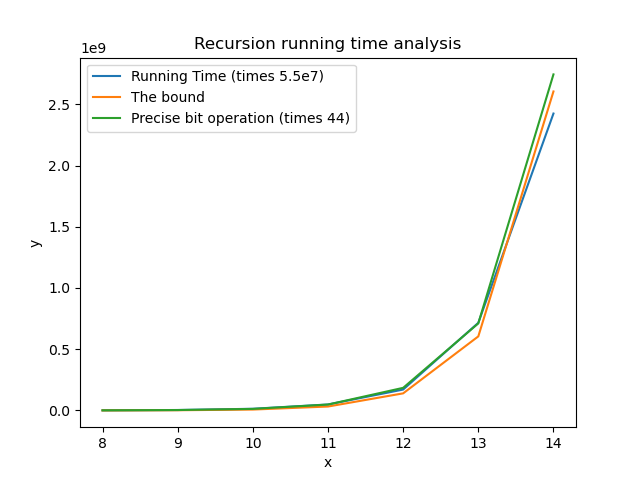
\includegraphics[width=100mm]{Figure_1.png}\scriptsize\par
	Figure 3.1: Running time analysis of recursion algorithm
	\end{center}
	\begin{center}
	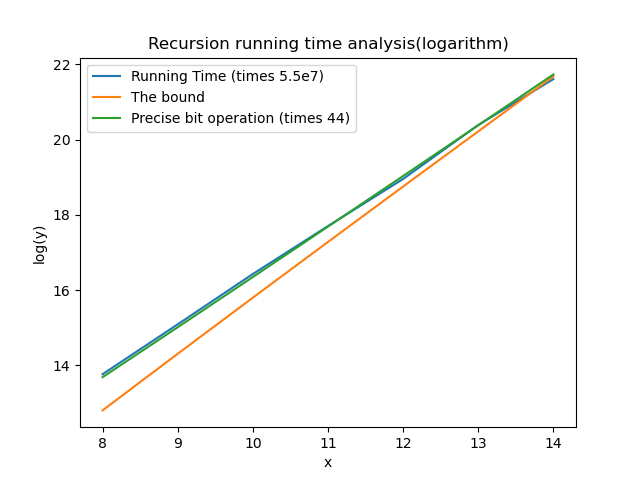
\includegraphics[width=100mm]{Figure_2.png}\scriptsize\par
	Figure 3.2: Running time analysis of recursion algorithm(logarithm)
	\end{center}
\end{problem}

\begin{problem}{4}
    \statement
    [A Dynamic Programming Algorithm for the Binomial Coefficient]
    Using pseudocode, write a dynamic programming algorithm
    computing ${n \choose k}$. Implement it in python! What is it running time
    in terms of $n$ and $k$?
    Would you say your algorithm is efficient? Why or why not?
    \solution
\begin{python}
# Dynamic Programming Algorithm for the Binomial Coefficient
def DP(n,k):
    if k < 0 or k > n: return 0
    f=[[0 for i in range(k+1)] for j in range(n+1)]
    f[0][0] = 1
    for i in range(1, n+1):
        f[i][0] = 1
        for j in range(1, k+1):
            f[i][j]=f[i-1][j]+f[i-1][j-1]
    return f[n][k]
\end{python}
    
	For calculating ${n \choose k}$, the dynamic programming algorithm runs $n k$ iterations.
	
	For each iteration, if $f_{i-1,j}$ and $f_{i-1,j-1}$ have at most $m$ bits, then the running time of adding will be $O(m)$.
    
	According to the previous task that proved ${n \choose k}=O((\frac{en}{k})^k)$, any element we need is at most $O(k\log(\frac{en}{k}))$ bits.
	So the total running time will be $O(k^2n\log(\frac{n}{k}))$.
    
    It's a rather better algorithm than the recursive one because it only calculate every ${n \choose k}$ once.
	
	We now use `measure\_alg' to find the real running time of the algorithm. To compare, we use the bound $k^2n\log(\frac{n}{k})$.

	Empirically we can announce that when $n, k$ grow twice, running time grows greater than $4$ times but less than $5$ times (the last one is slower mainly because it consumes more than 10 GB of memory). So there should be better bound for the question.
	% Table generated by Excel2LaTeX from sheet 'Sheet1'
\begin{table}[htbp]
	\centering
	  \begin{tabular}{cccc}
	  $x$ for ${2x \choose x}$ &    Running time(s) & Growth of running time   & Bound \\
	  $128$&$0.004472$&$N/A$&$3.63 \times 10^{ 5 }$\\
$256$&$0.010103$&$2.258921$&$2.91 \times 10^{ 6 }$\\
$512$&$0.034257$&$3.390872$&$2.33 \times 10^{ 7 }$\\
$1024$&$0.151667$&$4.42729$&$1.86 \times 10^{ 8 }$\\
$2048$&$0.674162$&$4.445015$&$1.49 \times 10^{ 9 }$\\
$4096$&$3.118444$&$4.62566$&$1.19 \times 10^{ 10 }$\\
$8192$&$19.49038$&$6.250034$&$9.53 \times 10^{ 10 }$\\
	  \end{tabular}%
	\par\scriptsize Table 4.1: Running time analysis of DP algorithm
  \end{table}%
  \begin{center}
	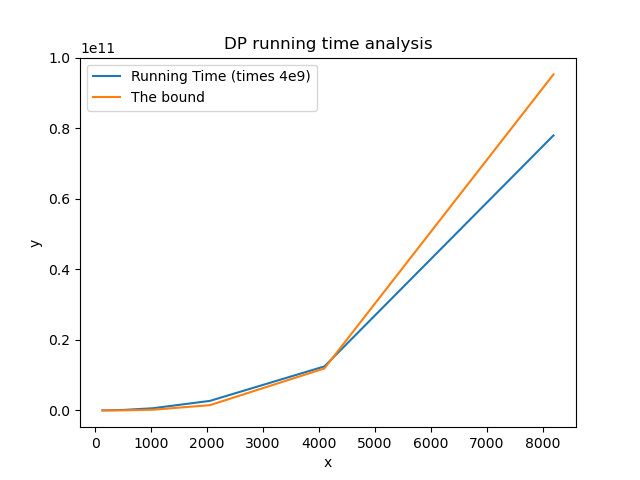
\includegraphics[width=100mm]{Figure_3.png}\scriptsize\par
	Figure 4.1: Running time analysis of DP algorithm
	\end{center}
	\begin{center}
	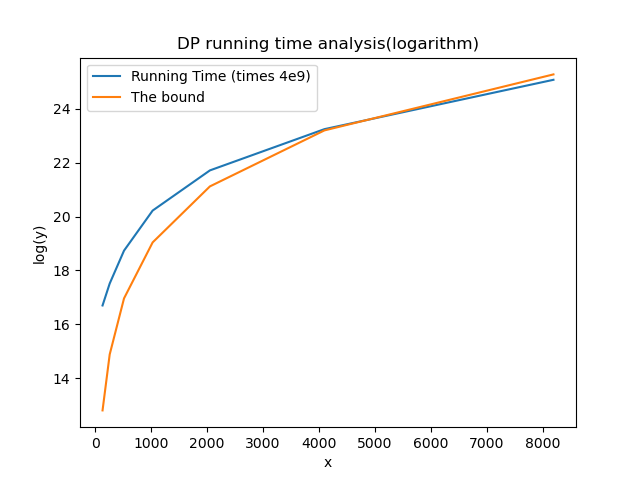
\includegraphics[width=100mm]{Figure_4.png}\scriptsize\par
	Figure 4.2: Running time analysis of recursion algorithm(logarithm)
	\end{center}
\end{problem}

\begin{problem}{5}
    \statement
    Suppose we are only interested in whether ${n \choose k}$ is even or odd,
  i.e., we want to compute ${n \choose k}  \mod 2$. You could do this by computing 
  ${n \choose k}$ using dynamic programming and then taking
  the result modulo $2$. What is the running time? Would you say this algorithm
  is efficient? Why or why not?
  \solution
If we first calculate ${n \choose k}$ in completely the same way of the previous task and take the last bit of the answer as the answer of this task, then the running time will still be the same as previous. It can't be a good algorithm because all we care is the last bit of the answer, but we use many time to calculate the useless higher bits.

For a better complexity, for each $f_{i, j}$ we only concern the lowest bit, so the complexity of multiplication and addition is $\Theta(1)$ because they are equivalent to bit AND and bit OR. In this case, the total complexity is $\Theta(nk)$.

However, we have a more efficient  -- $\Theta (\log n)$ -- conclusion: 
$$ {n \choose k} \bmod 2 = [n \wedge k = k]$$
where $\wedge$ is the bitwise AND operation.
	\begin{proof}
		$n \wedge k$ can't be $k$ when $k > n$, which means the assumption holds when $k > n$.
		All we need to concern is the situation that $0 \leq n \leq k$.

		According to the Lucas' Theorem, 
		
		\[
			{n \choose k}\equiv{{n \bmod p} \choose {k \bmod p}}{{ \lfloor n/p\rfloor} \choose { \lfloor k/p\rfloor}}(\bmod p)
		\]
		
		For $p=2$ and $n=(a_u....a_2a_1)_2$, $k=(b_v....b_2b_1)_2$. Note that $u \geq v$ since $n \leq k$, so we can apply Lucas' Theorem on it $v$ times, that is
		\begin{align*}
			{n \choose k} &\equiv {(a_u....a_2)_2 \choose (b_v....b_2)_2}{a_1 \choose b_1}\mod 2\\
			&\equiv {(a_u....a_3)_2 \choose (b_v....b_3)_2}{a_2 \choose b_2}{a_1 \choose b_1}\mod 2 \\
			&\equiv ...\\	
			&\equiv {(a_u....a_{v+1})_2 \choose 0}{a_v \choose b_v}...{a_1 \choose b_1}\mod 2\\
			&\equiv {a_v \choose b_v}...{a_1 \choose b_1}\mod 2
		\end{align*}		
		Because $a_i,b_i\in \{0,1\}$ and ${0 \choose 0}={0 \choose 1}={1 \choose 1}=1$, ${0 \choose 1}=0$, we have:
		
		\[
			\begin{split}
			{n \choose k} \bmod 2 = 1 &\Leftrightarrow {a_v \choose b_v}...{a_1 \choose b_1}\bmod 2=1 \\
			&\Leftrightarrow \forall i \in [v], {a_i \choose b_i}=1\\
			&\Leftrightarrow \forall i \in [v], (b_i=1\implies a_i=1)\\
			&\Leftrightarrow n \wedge k = k
			\end{split}
		\]		
    \end{proof}
\end{problem}

\begin{problem}{6}
    \statement
    Remember the ``period'' algorithm for computing $F'_n := (F_n \mod k)$ discussed in class:
    Find some $i,j$ between $0$ and $k^2$ for which 
    $F'_{i} =  F'_{j}$ and $F'_{i+1} = F'_{j+1}$. 
    Then for $d := j-i$ the sequence $F'_{n}$ will repeat every $d$ steps, as there will be a cycle.
    
    Show that a lasso cannot happen. That is, show 
    that the smallest $i$ for which this happens is $0$, i.e, for some $j$ we have
    $F'_0 = F'_j$ and $F'_1 = F'_{j+1}$ and thus $F'_n = F'_{n \text{ mod }  j}$.
    \solution
	\begin{proof}
	We prove this by contradiction.

	Suppose the smallest $i$ in some $(i, j)$ where $i < j$ that satisfies the above condition is greater than $0$.
	By definition of fibonacci number,
	$$F_{i-1} \equiv  F_{i+1}-F_i(\textnormal{ mod }  k)$$
	and similarly
	$$F_{j-1} \equiv  F_{j+1}-F_j(\textnormal{ mod }  k)$$
	
	Because $F_i = F_j$ and $F_{i+1} = F_{j+1}$, we have 
	$$F_{j-1} \equiv F_{i-1}(\textnormal{ mod }  k)$$
	and equivalently
	$$F'_{i-1} = F'_{j-1}$$

	We take $i^\prime = i - 1, j^\prime = j - 1$, then $(i^\prime, j ^ \prime)$ satisfies the preseted condition. Notice that $i^\prime < i$, thus this leads to contradiction.
	\end{proof}
\end{problem}

\end{document}
